\chapter{Alcuni prerequisiti matematici nell'ambito della computer vision}
\label{chap:math-prerequisites}


\section{Immagini digitali}
\label{sec:math-images}
Un'immagine digitale \textit{I} con risoluzione $m\times n$ ($width \times height$) \`e una matrice di valori interi di $n$ righe e $m$ colonne, che pu\`o essere matematicamente interpretata come una funzione semplice (n\'e iniettiva, n\'e suriettiva) 
\begin{equation}
	I: \mathbb{N}\times\mathbb{N}\supseteq X \to P\subseteq \mathbb{N}^{c},
	\label{eq:digital-image-function}
\end{equation}
che si occupa di mappare una coppia ordinata $(u,v)\in\mathbb{N}\times\mathbb{N}$, con $u,v\in\mathbb{N}$, in una \textit{c-upla} $p=(p_{1}, p_{2}, \dots, p_{c})\in\mathbb{N}^{c}$, in cui ciascun $p_{i}$ di $p$ rappresenta il valore del pixel in posizione $(u,v)$ nel canale ${i}$ dell'immagine, con $0 \leq p_{i} \leq 2^{b} - 1$, dove $b$ \`e il numero fissato di bit utilizzati per rappresentare ciascun pixel e $2^{b}$ indica il massimo numero di colori o di livelli di grigio rappresentabili.\par
Per esempio, ipotizzando di utilizzare canali colore standard, nel caso in cui si lavori con immagini in scala di grigi si avr\`a $c=1$, mentre nel caso in cui si lavori con immagini \textit{RGB} si avr\`a $c=3$ ($c=4$ per immagini \textit{RGBA} o \textit{CMYK}). Inoltre, supponendo di utilizzare una profondit\`a pari a $b=8$ sar\`a possibile specificare interi compresi tra $0$ e $255$ per i valori di ciascun pixel.


\section{Convoluzione}
\label{sec:math-convolution}
La \textit{convoluzione} \`e un'operazione alla base dell'\textit{image processing}, grazie alla quale \`e possibile analizzare ed eventualmente accentuare o alleviare diversi aspetti di una data immagine, come la sfocatura, la nitidezza, i contorni e molto altro. L'operazione, che viene descritta nella forma discreta, prende in input due immagini digitali, ovvero l'immagine originale \textit{I} (normalmente a singolo canale) e l'immagine $K$, denominata \textit{kernel}, e intuitivamente si occupa di far scorrere la matrice $K$ sull'immagine $I$, generalmente a partire dal pixel in alto a sinistra, effettuando una somma pesata dei valori di $I$ dati dalle proiezioni delle posizioni correntemente analizzate dalla matrice $K$, in cui i pesi sono dati proprio dagli elementi di $K$. Solitamente la dimensione della matrice $K$ \`e molto minore della dimensione dell'immagine originale e spesso $K$ \`e una matrice quadrata $n\times n$, con $n$ dispari.\par
Pi\`u formalmente, come descritto in \cite{bib:convolution}, l'operazione di \textit{convoluzione} $I * K$ in un punto $(i,j)$ \`e data da:
\begin{equation}
	\label{eq:convolution}
	\begin{split}
		I^{*}(i, j) & = \sum_{x = -n}^{n}\sum_{y = -n}^{n}(I(i-x, j-y)\cdot K(x,y))=\\
		& = \sum_{x = 1}^{n}\sum_{y = 1}^{n}(I(i + \left\lceil{\dfrac{n}{2}}\right\rceil - x, j + \left\lceil{\dfrac{n}{2}}\right\rceil - y)\cdot K(x,y))
	\end{split}
\end{equation}
Nel caso in cui nella formula \ref{eq:convolution} i segni \textit{-} e \textit{+} venissero invertiti si otterrebbe la formulazione della \textit{correlazione} $I \otimes K$ in un punto $(i,j)$:
\begin{equation}
	\label{eq:correlation}
	\begin{split}
		I^{\otimes}(i, j) & = \sum_{x = -n}^{n}\sum_{y = -n}^{n}(I(i+x, j+y)\cdot K(x,y))=\\
		& = \sum_{x = 1}^{n}\sum_{y = 1}^{n}(I(i - \left\lceil{\dfrac{n}{2}}\right\rceil + x, j - \left\lceil{\dfrac{n}{2}}\right\rceil + y)\cdot K(x,y))
	\end{split}
\end{equation}\par
\textit{Convoluzione} e \textit{correlazione} possono risultare equivalenti se per passare da un'operazione all'altra si effettua un ribaltamento orizzontale e verticale del filtro (graficamente $K$ viene ruotata di $180^{\circ}$). Dunque le due operazioni risultano identiche nel caso in cui la matrice $K$ sia simmetrica rispetto ai due assi. Nella pratica, si preferisce utilizzare la \textit{convoluzione} quando sono necessarie le propriet\`a commutativa, associativa e distributiva. Inoltre, dato che spesso il risultato delle operazioni descritte viene utilizzato come valore di intensit\`a di pixel, tale risultato viene normalizzato, dividendolo per la somma dei pesi del filtro.\par
La complessit\`a computazionale delle operazioni, data ad esempio un'immagine di dimensione $m\times m$ e un kernel di dimensione $n\times n$, \`e piuttosto elevata, dato che richiede un numero di moltiplicazioni pari a $n^{2}\cdot m^{2}$ e altrettante somme.\par
Di seguito un esempio di \textit{convoluzione} e \textit{correlazione}, riportato in \cite{bib:convolution}:
$$
I=\bordermatrix{
		& & & j & & \cr
        & & & \dots & & \cr
		& & 30 & 28 & 32 & \cr
		i & \vdots & 27 & 26 & 10 & \vdots \cr
		& & 29 & 22 & 18 & \cr
		& & & \dots & & \cr
	},
K=\begin{pmatrix} 
	4 & -2 & 1 \\
	-1 & 5 & -3\\
	-6 & 0 & 4
\end{pmatrix}
$$
Calcoliamo $I * K$ nella posizione $(i, j)$ come 
\begin{equation}
	\label{eq:convolution-example}
	\begin{split}
		I^{*}(i, j) & = 18\cdot 4 - 22\cdot 2 + 29\cdot 1 - 10\cdot 1+\\ 
		& + 26\cdot 5 -27\cdot 3 - 32\cdot 6 + 28\cdot 0 + 30\cdot 4 = 24,
	\end{split}
\end{equation}
mentre calcoliamo $I \otimes K$ nella posizione $(i, j)$ come 
\begin{equation}
	\label{eq:correlation-example}
	\begin{split}
		I^{\otimes}(i, j) & = 30\cdot 4 - 28\cdot 2 + 32\cdot 1 - 27\cdot 1+\\
		& + 26\cdot 5 -10\cdot 3 - 29\cdot 6 + 22\cdot 0 + 18\cdot 4 = 67
	\end{split}
\end{equation}\par
Un problema che pu\`o risultare evidente riguarda il modo di trattare i bordi, nel caso in cui l'intorno di un pixel non sia disponibile. Per ovviare a tale problema esistono diverse tecniche valide, come ipotizzare che i pixel non disponibili abbiano intensit\`a zero, oppure prolungare i pixel di bordo supponendo intensit\`a costante in quelli non disponibili.\par
Alcuni esempi di filtri classici:
\begin{itemize}
	\item Sfocatura (filtro di \textit{Gauss}): $\begin{pmatrix} 
		1 & 2 & 1 \\
		2 & 4 & 2\\
		1 & 2 & 1
	\end{pmatrix}$
	\item Nitidezza: $\begin{pmatrix} 
		0 & -1 & 0 \\
		-1 & 5 & -1\\
		0 & -1 & 0
	\end{pmatrix}$
	\item Contorni (filtro di \textit{Laplace}): $\begin{pmatrix} 
		-1 & -1 & -1 \\
		-1 & 8 & -1\\
		-1 & -1 & -1
	\end{pmatrix}$
\end{itemize}\par
In figura \ref{fig:gauss-filter} \`e possibile osservare un esempio di sfocatura di un'immagine, tramite l'applicazione di un filtro di \textit{Gauss}.
\begin{figure}[H]
	\centering
	\resizebox{.7\textwidth}{!}{
		\centering
		\subfloat[Input] {%
			\scalebox{0.5}[0.5] {
				\frame{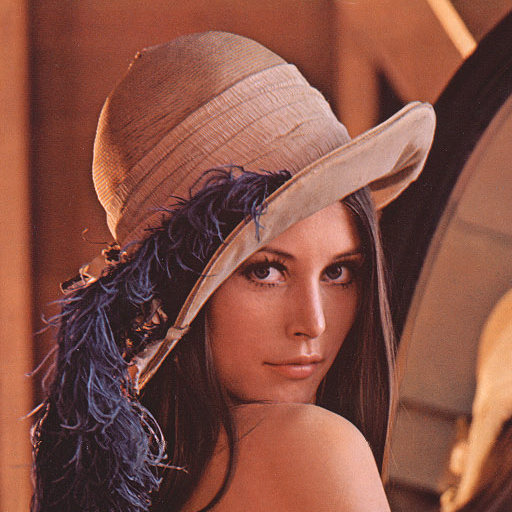
\includegraphics[width=.8\linewidth]{img/lena.png}}
			}
		}
		\subfloat[Output] {%
			\scalebox{0.5}[0.5] {
				\frame{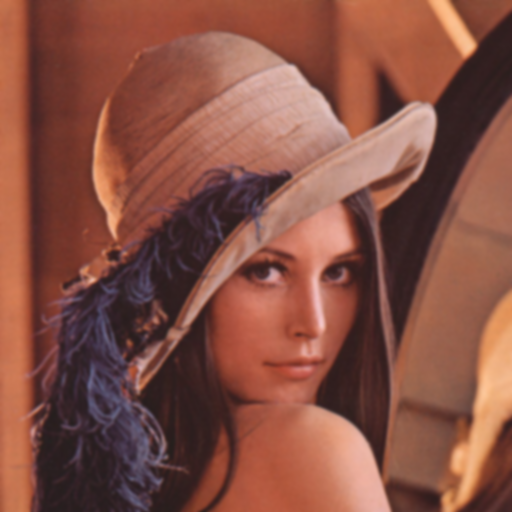
\includegraphics[width=.8\linewidth]{img/lena-blurred.png}}
			}
		}
	}
	\caption{Applicazione di un filtro di \textit{Gauss} di dimensione $10\times10$} \label{fig:gauss-filter}
\end{figure}


\section{Elementi di morfologia}
\label{sec:math-morph}

\subsection{Basi della matematica morfologica}
\label{subsec:math-morph-basis}
La matematica morfologica \`e una collezione di operatori, basata sulla teoria degli insiemi e definita su una struttura astratta\footnote{La struttura astratta alla quale si fa riferimento \`e un \textit{reticolo} infinito, un'estensione della teoria degli insiemi di Minkowski.}. Il suo obiettivo \`e quello di analizzare le forme e gli oggetti di un'immagine digitale, attraverso trasformazioni quali erosione, dilatazione, apertura, chiusura e altre. Nella loro forma originaria le operazioni morfologiche prevedono l'utilizzo di un'\textit{immagine binaria} a singolo canale, composta da pixel che possono assumere solo due valori, 1 e 0, bianco e nero, \textit{foreground} e \textit{background}, oltre che di un \textit{elemento strutturante} (\textit{SE}), anch'esso sotto forma di immagine binaria a singolo canale, generalmente di dimensione molto minore di quella dell'immagine originale. Per correttezza, come effettuato in \cite{bib:digital-image-processing}, da ora in poi, in questa sezione, considereremo un'immagine binaria \textit{I} anche come un insieme di punti $Q_{I}$ contenente tutte le coppie $(u,v)$ di pixel \textit{foreground} di \textit{I}, ovvero tali che $I(u, v) = 1$ e considereremo i termini in \textbf{grassetto} come coppie ordinate $(u,v) \in \mathbb{N}\times\mathbb{N}$.
\newpage
Il risultato dell'operazione di \textit{erosione} di un'immagine mostra dove lo SE viene contenuto negli oggetti dell'immagine, ovvero, intuitivamente permette di rimuovere pixel dal contorno di \textit{componenti connesse}\footnote{Una \textit{componente connessa} \textit{C} di un insieme di punti \textit{foreground} $P$ di un'immagine binaria $I$ \`e un insieme $C\subseteq P$ tale che $\forall \textbf{p}_{i}, \textbf{p}_{j} \in C$ esiste un percorso $\textbf{p}_{i}, \dots, \textbf{p}_{j}$ in cui ogni $\textbf{p}_{h}$ \`e \textit{k-vicino} (\textit{4-vicino} o \textit{8-vicino}) a $\textbf{p}_{h-1}$ e $\neg \exists \textbf{q}\notin P$ \textit{k-adiacente} a un punto di $P$ \cite{bib:binary-images-connectivity}.} di colore bianco, in quantit\`a dipendente dalla grandezza dello SE. In formule, come riportato in \cite{bib:top-hat-paper}:
\begin{equation}
	\label{eq:erosion}
	[\epsilon_{Q_{SE}}(I)](\textbf{x}) = \underset{\textbf{s}\in Q_{SE}}{\bigwedge}(I(\textbf{x}+\textbf{s}))
\end{equation}\par
Il risultato dell'operazione di \textit{dilatazione} di un'immagine mostra dove lo SE tocca gli oggetti dell'immagine, ovvero, intuitivamente permette di aggiungere pixel al contorno di componenti connesse di colore bianco, in quantit\`a dipendente dalla grandezza dello SE. In formule, come riportato in \cite{bib:top-hat-paper}:
\begin{equation}
	\label{eq:dilation}
	[\delta_{Q_{SE}}(I)](\textbf{x}) = \underset{\textbf{s}\in Q_{SE}}{\bigvee}(I(\textbf{x}+\textbf{s}))
\end{equation}\par
In figura \ref{fig:erosion-dilation} \`e possibile osservare l'applicazione degli operatori di \textit{erosione} e \textit{dilatazione}, con input-output in ordine sinistra-destra e destra-sinistra, rispettivamente.
\begin{figure}[h]
	\centering
	\hspace*{15.0pt}
	\subfloat[Prima (dopo)] {
		\resizebox{6cm}{5cm}{%
		\begin{tikzpicture}[framed,background rectangle/.style={draw=black,fill=black},scale=1.5]
			\draw [fill=white] plot [smooth cycle] coordinates {(0,0) (1,1) (3,1) (1,0) (2,-1)};
		\end{tikzpicture}
		}
	}
	\subfloat[Dopo (prima)] {
		\resizebox{6cm}{5cm}{%
		\begin{tikzpicture}[framed,background rectangle/.style={draw=black,fill=black},scale=1.5]
			\draw [fill=white,scale=0.3] plot [smooth cycle] coordinates {(0,0) (1,1) (3,1) (1,0) (2,-1)};
		\end{tikzpicture}
		}
	}
	\caption{Erosione (dilatazione) con elemento strutturante rettangolare} \label{fig:erosion-dilation}
\end{figure}

Le operazioni di \textit{apertura} (\textit{chiusura}) sono invece la combinazione in sequenza di erosione (dilatazione) e dilatazione (erosione) dello SE con la propria \textit{riflessione}\footnote{La \textit{riflessione} di un insieme di punti $P$ di un'immagine binaria $I$ rispetto all'origine viene definita come $\check{P}=\{(-u,-v) \colon (u,v)\in P\}$ \cite{bib:digital-image-processing}.}. Queste due operazioni vengono molto utilizzate per rimuovere "sporco" (\textit{noise}) dalle immagini e per "chiudere" piccoli "buchi" all'interno di oggetti che si trovano nel \textit{foreground}. In formule, come riportato in \cite{bib:top-hat-paper}:
\begin{equation}
	\label{eq:opening}
	\gamma_{Q_{SE}}(I) = \delta_{\check{Q_{SE}}}(\epsilon_{Q_{SE}}(I)),
\end{equation}
\begin{equation}
	\label{eq:closing}
	\phi_{Q_{SE}}(I) = \epsilon_{\check{Q_{SE}}}(\delta_{Q_{SE}}(I))
\end{equation}\par
In figura \ref{fig:opening} \`e possibile osservare la rimozione delle aree \textit{foreground} di piccola dimensione, grazie all'utilizzo dell'\textit{apertura} morfologica.
\begin{figure}[h]
	\centering
	\subfloat[Prima] {
		\begin{tikzpicture}[framed,background rectangle/.style={draw=black,fill=black},scale=0.8]
			\draw [fill=white] plot [smooth cycle] coordinates {(0,0) (1,1) (3,1) (1,0) (2,-1)};
			\draw [fill=white] plot [smooth cycle] coordinates {(4,0) (4,2) (7,0) (5,0) (5,-2)};
			\draw [fill=white] (4,3) circle (0.1cm);
			\draw [fill=white] (3,2) circle (0.2cm);
			\draw [fill=white] (1,-2) circle (0.15cm);
			\draw [fill=white] (7,-2) circle (0.08cm);
		\end{tikzpicture}
	}
	\subfloat[Dopo] {
		\begin{tikzpicture}[framed,background rectangle/.style={draw=black,fill=black},scale=0.8]
			\draw [fill=white] plot [smooth cycle] coordinates {(0,0) (1,1) (3,1) (1,0) (2,-1)};
			\draw [fill=white] plot [smooth cycle] coordinates {(4,0) (4,2) (7,0) (5,0) (5,-2)};
			\draw [fill=black] (4,3) circle (0.1cm);
			\draw [fill=black] (1,-2) circle (0.15cm);
		\end{tikzpicture}
	}
	\caption{Apertura morfologica con elemento strutturante circolare} \label{fig:opening}
\end{figure}

\subsection{Ricostruzione morfologica}
\label{subsec:math-morph-reconstruction}
La \textit{ricostruzione} \`e un'operazione molto utile nella matematica morfologica, che viene spesso presentata come un insieme di operatori \textit{geodetici}, che consentono di estrarre le componenti connesse dell'immagine originale, marcate da un'altra immagine \textit{marker}. Gli operatori di \textit{erosione} e \textit{dilatazione} possono dunque essere ridefiniti in senso \textit{geodetico}. In particolare, consideriamo al solito un'immagine binaria \textit{I} (\textit{mask}), definita dal suo insieme di punti \textit{foreground} $Q_{I}$, un elemento strutturante (SE), che definisce la connettivit\`a da rispettare, e un'immagine \textit{marker} \textit{F} tale che $Q_{F} \subseteq Q_{I}$, che permette di definire quali componenti connesse devono subire i risultati delle operazioni morfologiche. Come riportato in \cite{bib:binary-image-analysis}, definiamo l'\textit{erosione condizionale} come:
\begin{equation}
	\label{eq:conditional-erosion}
	[\epsilon_{Q_{SE}}(F)]^{(0)}_{I}(\textbf{x}) = [\epsilon_{Q_{SE}}(F)](\textbf{x}) \vee I(\textbf{x})
\end{equation}
e la \textit{dilatazione condizionale} come:
\begin{equation}
	\label{eq:conditional-dilation}
	[\delta_{Q_{SE}}(F)]^{(0)}_{I}(\textbf{x}) = [\delta_{Q_{SE}}(F)](\textbf{x}) \wedge I(\textbf{x})
\end{equation}
Le varianti \textit{geodetiche}, descritte in \cite{bib:top-hat-paper}, vengono definite in modo iterativo a partire da quelle \textit{condizionali}. Dunque, si avr\`a che l'\textit{erosione geodetica} pu\`o essere espressa come:
\begin{equation}
	\label{eq:geodesic-erosion}
	[\epsilon_{Q_{SE}}(F)]^{(i)}_{I}(\textbf{x}) = [\epsilon_{Q_{SE}}([\epsilon_{Q_{SE}}(F)]^{(i-1)}_{I}(\textbf{x}))]^{(0)}_{I}(\textbf{x}), i=1,2,3,\dots,
\end{equation}
mentre la \textit{dilatazione geodetica}:
\begin{equation}
	\label{eq:geodesic-dilation}
	[\delta_{Q_{SE}}(F)]^{(i)}_{I}(\textbf{x}) = [\delta_{Q_{SE}}([\delta_{Q_{SE}}(F)]^{(i-1)}_{I}(\textbf{x}))]^{(0)}_{I}(\textbf{x}), i=1,2,3,\dots
\end{equation}
Concettualmente, le iterazioni sopra definite potrebbero continuare indefinitamente, ma per ragioni pratiche si sceglie di farle terminare per un intero \textit{n} tale che nessun cambiamento avvenga $\forall n' > n$. L'output stabile 
\begin{equation}
	\label{eq:erosion-reconstruction}
	R^{\epsilon}_{I}(F)=[\epsilon_{Q_{SE}}(F)]^{(n)}_{I}(\textbf{x}),
\end{equation}
\begin{equation}
	\label{eq:dilation-reconstruction}
	R^{\delta}_{I}(F)=[\delta_{Q_{SE}}(F)]^{(n)}_{I}(\textbf{x})
\end{equation}
cos\`i definito viene denominato rispettivamente \textit{erosione} e \textit{dilatazione} con \textit{ricostruzione} (vedi figura \ref{fig:dilation-reconstruction}).\par
\begin{figure}[H]
	\centering
	\resizebox{\textwidth}{!}{
		\centering
		\subfloat[Mask] {%
			\scalebox{0.5}[0.5] {
				\frame{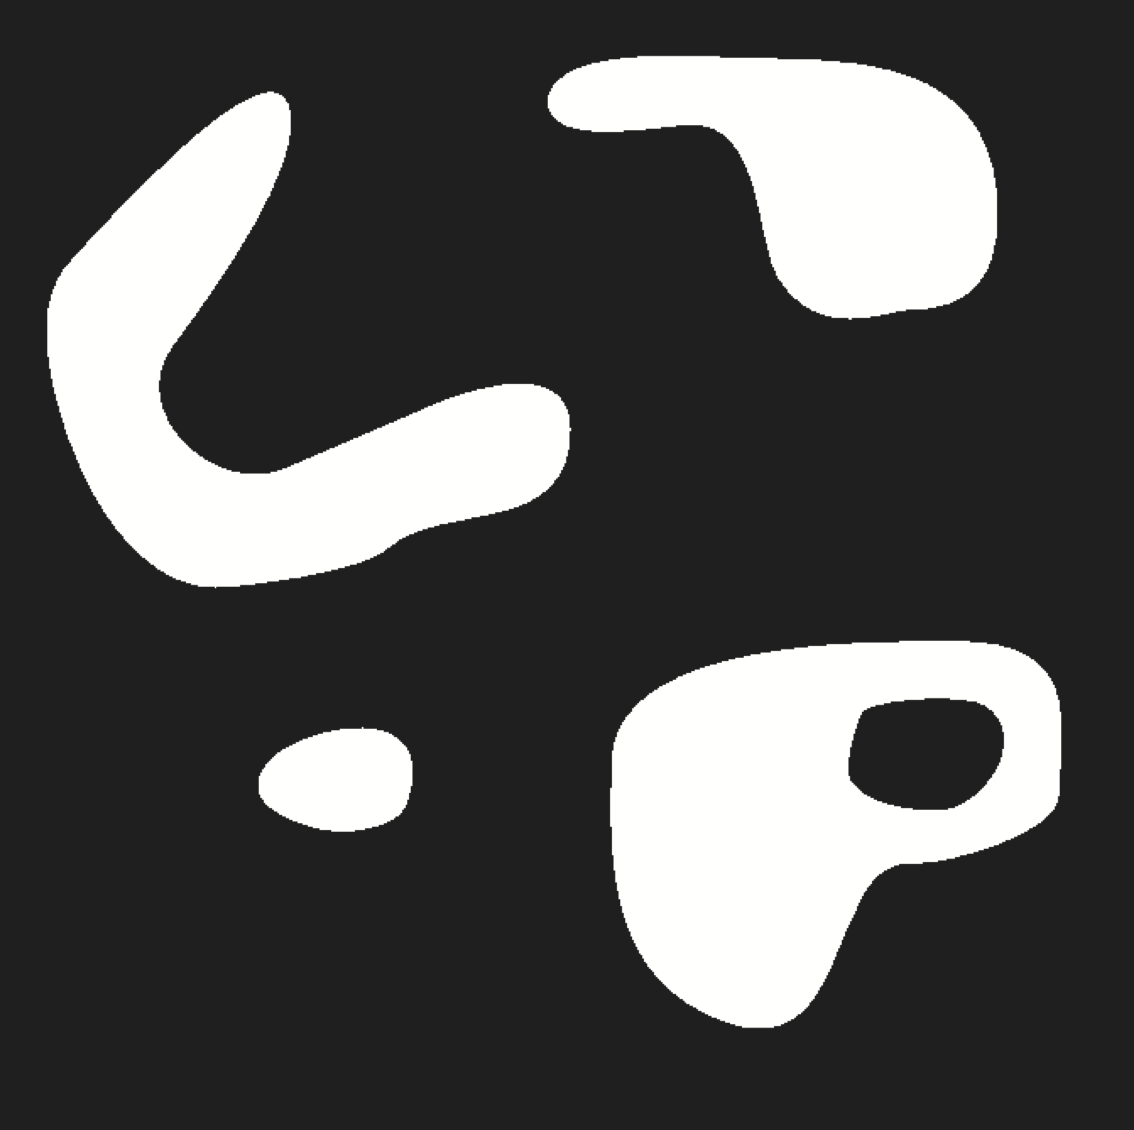
\includegraphics[width=.7\linewidth]{img/reconstruction-mask.png}}
			}
		}
		\subfloat[Marker] {%
			\scalebox{0.5}[0.5] {
				\frame{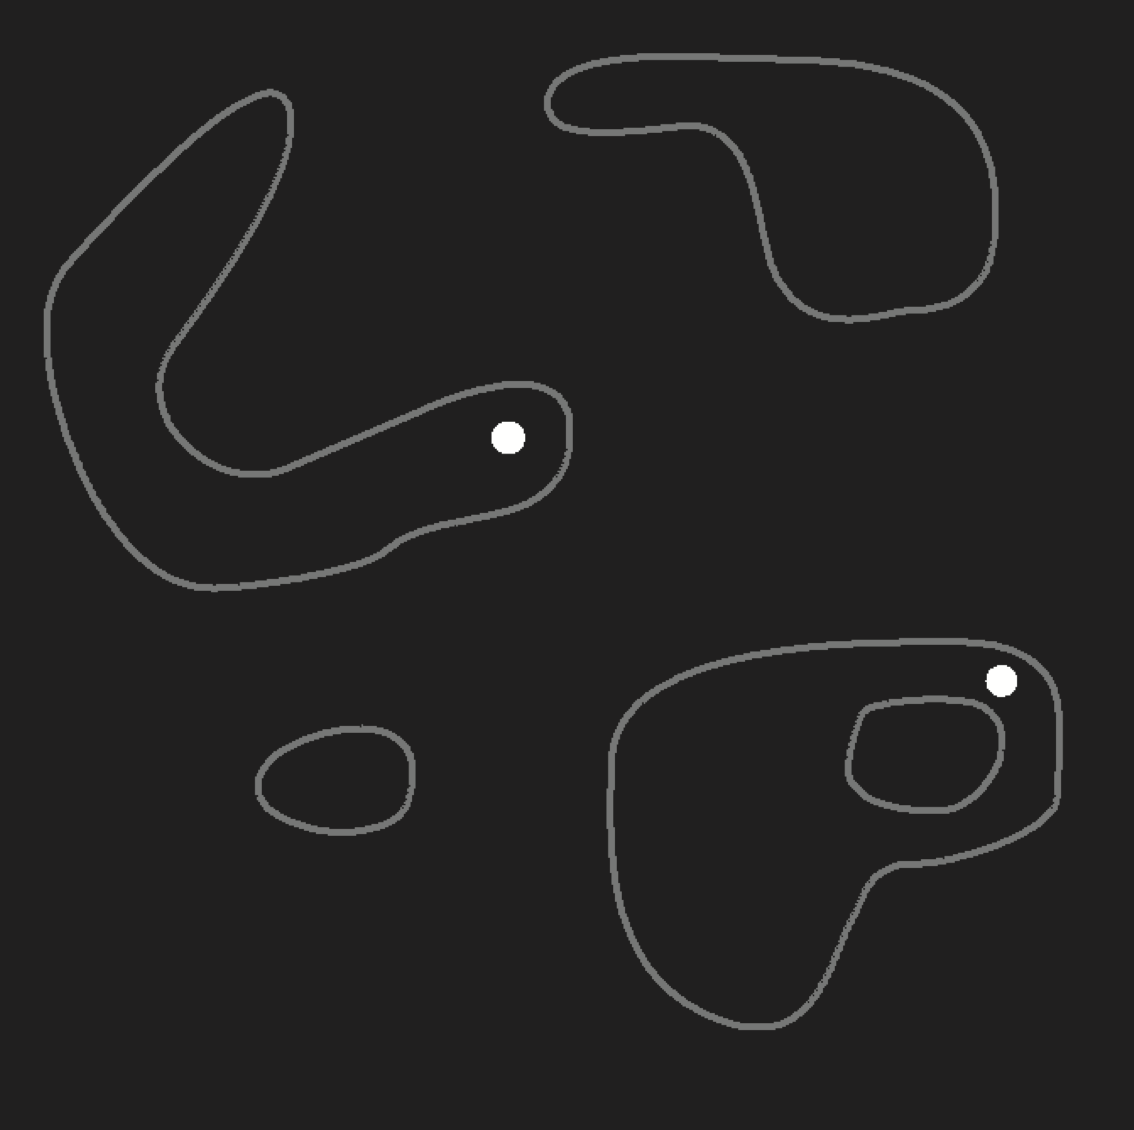
\includegraphics[width=.7\linewidth]{img/reconstruction-marker.png}}
			}
		}
		\subfloat[Output] {%
			\scalebox{0.5}[0.5] {
				\frame{
\includegraphics[width=.7\linewidth]{img/reconstruction-output.png}}
			}
		}
	}
	\caption[\textit{Dilatazione} con \textit{ricostruzione}]{\textit{Dilatazione} con \textit{ricostruzione}\protect\footnotemark} \label{fig:dilation-reconstruction}
\end{figure}
\enlargethispage{3\baselineskip}\footnotetext{\label{foot:advanced-morph}\textit{Fonte}: \emph{Advanced morphological image processing} \cite{bib:advanced-morphological}}

Definiamo adesso le operazioni di \textit{apertura} e \textit{chiusura} con \textit{ricostruzione}: l'operazione di apertura permette di rimuovere oggetti in base allo SE usato, ma ha il limite di non preservare le altre strutture, che potrebbero comunque venir modificate. Questo limite viene completamente superato dall'operatore di \textit{apertura} con \textit{ricostruzione}, che opera nel seguente modo: l'immagine viene erosa con lo SE come per l'apertura normale, ma invece di far seguire una dilatazione, si opera una ricostruzione usando l'immagine originale come \textit{mask}, e l'immagine erosa come \textit{marker}. L'operazione di \textit{chiusura} con \textit{ricostruzione} opera in modo analogo. In formule, come riportato in \cite{bib:top-hat-paper}:
\begin{equation}
	\label{eq:opening-reconstruction}
	\tilde{\gamma}_{R}(I) = \gamma_{R}^{(n)}(I) = R_{I}^{\delta}[\epsilon^{(n)}(I)],
\end{equation}
\begin{equation}
	\label{eq:closing-reconstruction}
	\tilde{\phi}_{R}(I) = \phi_{R}^{(n)}(I) = R_{I}^{\epsilon}[\delta^{(n)}(I)]
\end{equation}\par
In figura \ref{fig:opening-reconstruction} \`e possibile osservare un confronto fra le operazioni di \textit{apertura} morfologica "standard" e con \textit{ricostruzione}, in cui l'obiettivo \`e quello di estrarre le lettere con altezza superiore a $50px$, tramite l'utilizzo di uno SE di dimensione $51\times1$.
\begin{figure}[H]
	\centering
	\resizebox{\textwidth}{!}{
		\centering
		\subfloat[Input] {%
			\scalebox{0.5}[0.5] {
				\frame{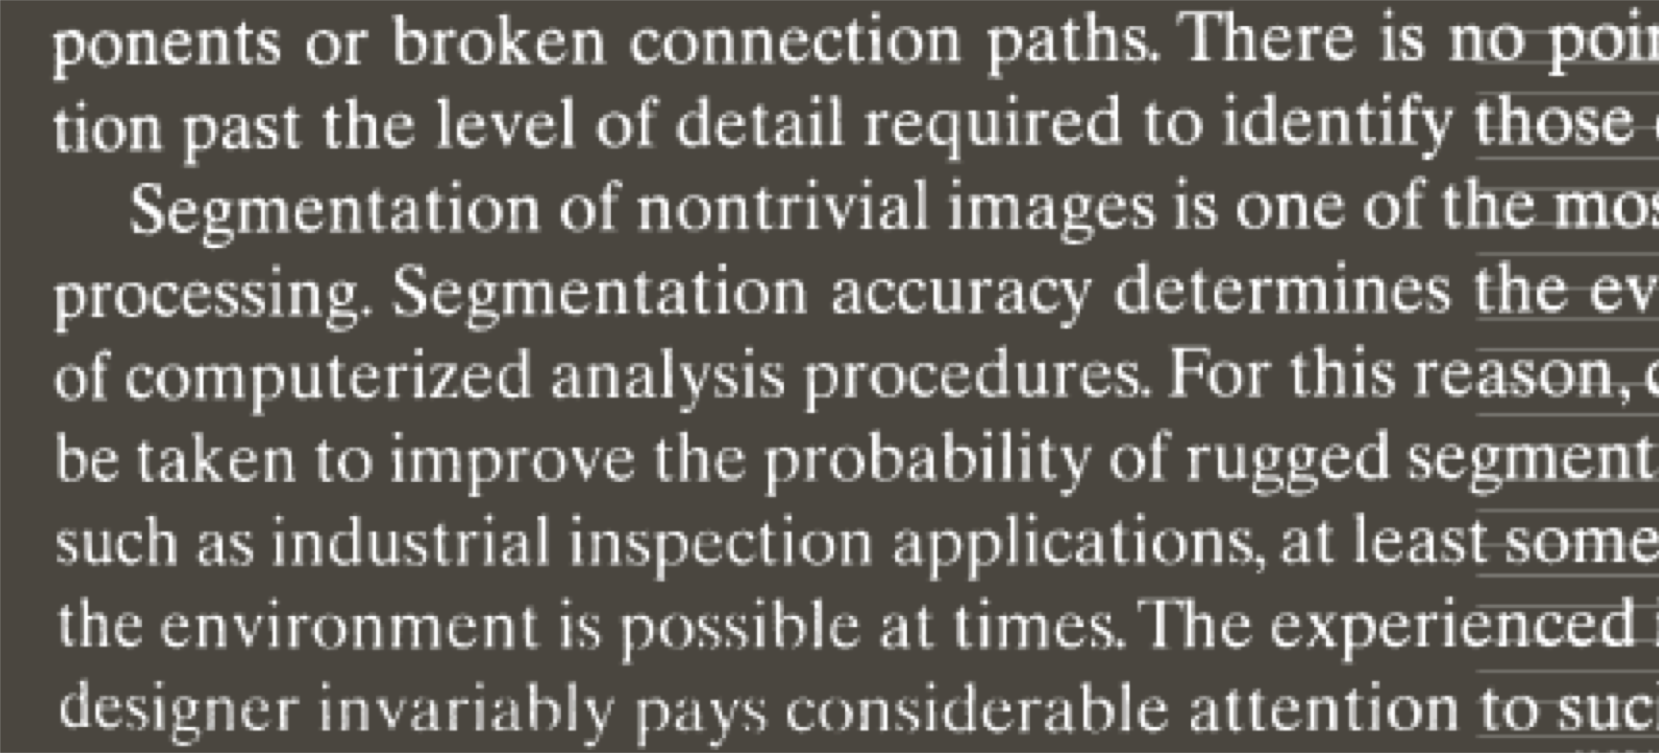
\includegraphics[width=.7\linewidth]{img/opening-reconstruction-input.png}}
			}
		}
		\subfloat[Output \textit{apertura}] {%
			\scalebox{0.5}[0.5] {
				\frame{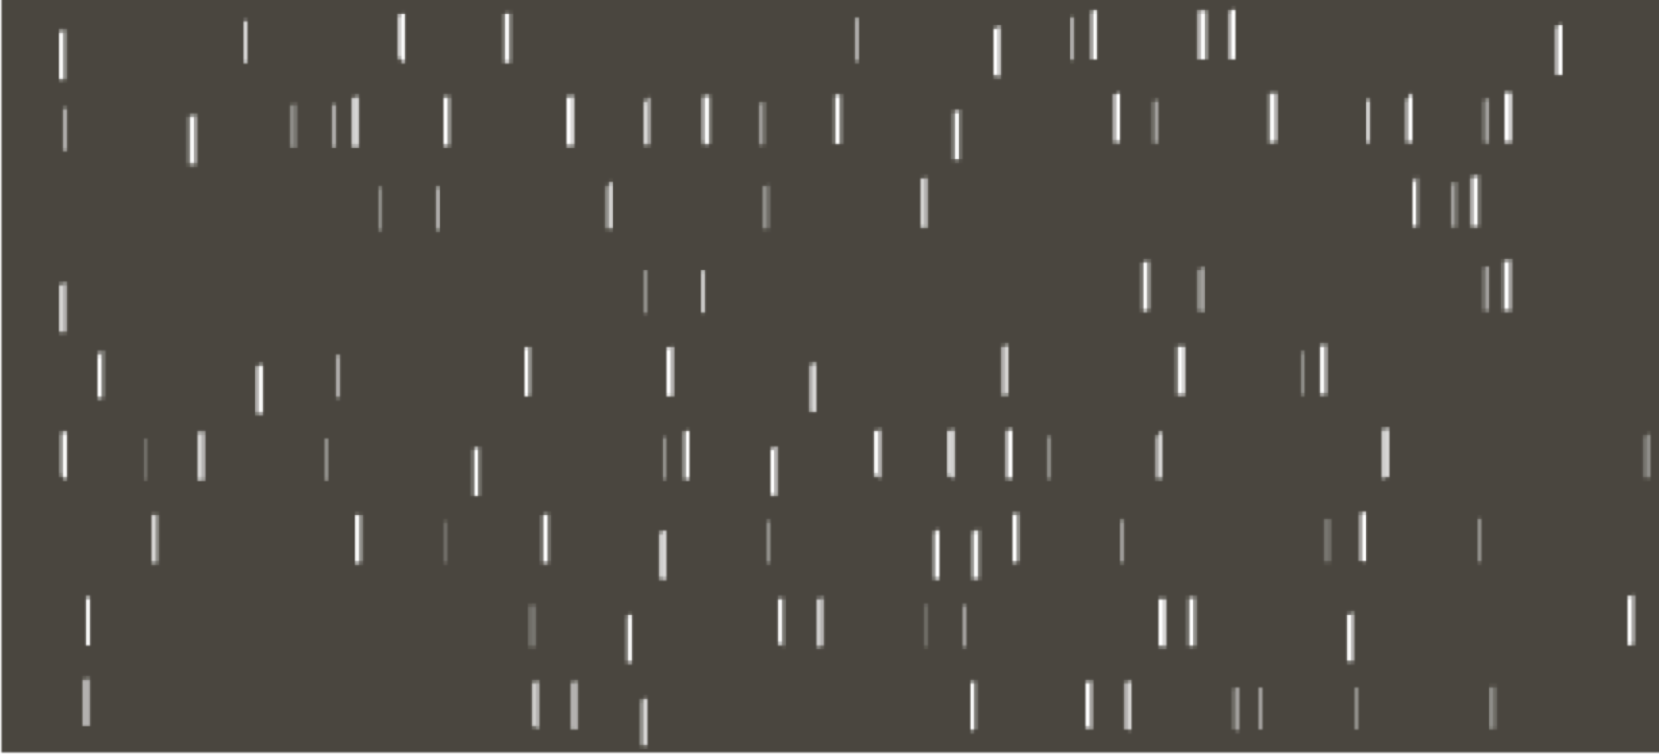
\includegraphics[width=.7\linewidth]{img/opening-output.png}}
			}
		}
		\subfloat[Output \textit{apertura} con \textit{ricostruzione}] {%
			\scalebox{0.5}[0.5] {
				\frame{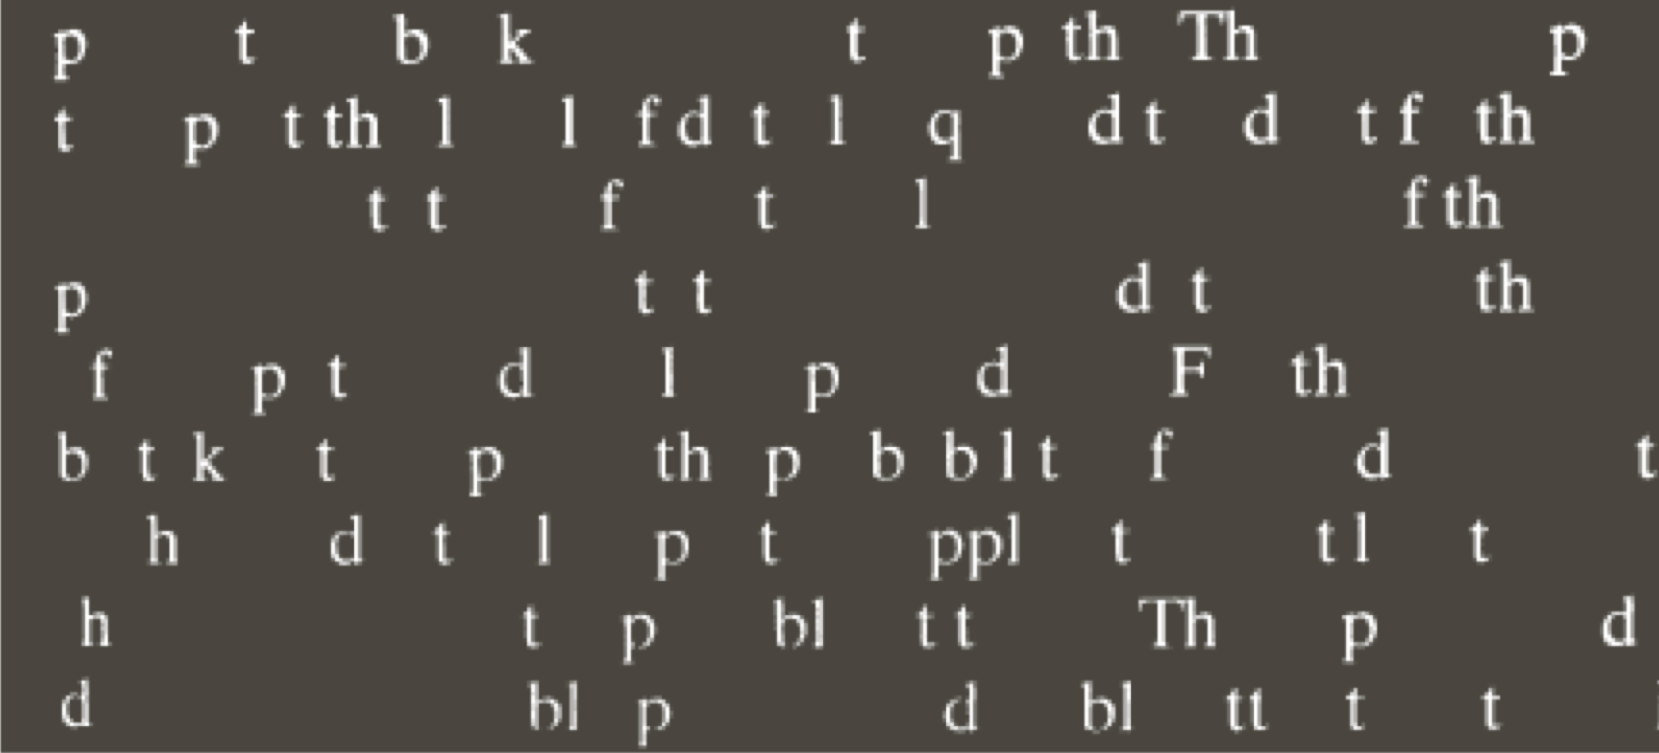
\includegraphics[width=.7\linewidth]{img/opening-reconstruction-output.png}}
			}
		}
	}
	\caption[\textit{Apertura} con \textit{ricostruzione}]{\textit{Apertura} con \textit{ricostruzione}\protect\footnotemark} \label{fig:opening-reconstruction}
\end{figure}
\footnotetext{Vedi nota \ref{foot:advanced-morph}}

\subsection{Altri operatori morfologici}
\label{subsec:math-morph-others}
Gli operatori finora descritti permettono di estrarre caratteristiche importanti all'interno delle immagini, ma, ad esempio, consentono difficilmente di effettuare un'equalizzazione di parametri dell'immagine, oppure di estrarre piccoli particolari d'interesse, oppure ancora di rilevare i contorni di un oggetto. Per ovviare a queste problematiche, si pu\`o ricorrere all'utilizzo di trasformazioni pi\`u specifiche, derivate da quelle di base. In particolare, possiamo definire l'operatore \textit{top-hat}, nelle due versioni \textit{bianca} e \textit{nera}, rispettivamente:
\begin{equation}
	\label{eq:white-top-hat}
	g_{Q_{SE}}^{w}(I) = I - \gamma_{Q_{SE}}(I),
\end{equation}
\begin{equation}
	\label{eq:black-top-hat}
	g_{Q_{SE}}^{b}(I) = \phi_{Q_{SE}}(I) - I
\end{equation}
Entrambi ritornano un'immagine contenente gli elementi dell'immagine originale che sono pi\`u piccoli dello SE. Il primo ritorna inoltre solo gli elementi pi\`u \textit{luminosi} degli oggetti a loro vicini, mentre il secondo solo gli elementi pi\`u \textit{scuri} degli oggetti a loro vicini. Questo ci fa capire che un buon utilizzo per questo operatore riguarda la correzione di condizioni di luce non uniforme all'interno di un'immagine, per consentire una separazione tra \textit{foreground} e \textit{background} pi\`u marcata, grazie al conseguente incremento di contrasto.
\par Altri operatori morfologici sono quello \textit{hit-or-miss}, che consente di estrarre pixel i cui vicini hanno una specifica configurazione (\textit{pattern}), in base allo SE utilizzato; oppure quello del \textit{gradiente}, che consiste nella differenza tra dilatazione ed erosione di un'immagine, e restituisce, ad esempio, i contorni di oggetti (vedi figura \ref{fig:morph-gradient}).
\begin{figure}[H]
	\centering
	\resizebox{.62\textwidth}{!}{
		\centering
		\subfloat[Input] {%
			\scalebox{0.5}[0.5] {
				\frame{
\includegraphics[width=.6\linewidth]{img/gradient-input.png}}
			}
		}
		\subfloat[Output] {%
			\scalebox{0.5}[0.5] {
				\frame{
\includegraphics[width=.6\linewidth]{img/gradient-output.png}}
			}
		}
	}
	\caption[\textit{Gradiente} morfologico]{\textit{Gradiente} morfologico\protect\footnotemark} \label{fig:morph-gradient}
\end{figure}
\footnotetext{\textit{Fonte}: \emph{OpenCV documentation} \cite{bib:opencv}}
